\documentclass{article}

 \IfFileExists{fontenc.sty}{%
   \usepackage[T1]{fontenc}}{}
\usepackage{mathptmx}
\usepackage[super]{nth}
\usepackage{graphicx}
\usepackage{url}
\usepackage{amssymb,amsmath}
\usepackage{manfnt}
\usepackage{xcolor}
\usepackage{layout}

\usepackage[text={6.9in,9in},%
    inner=0.8in,top=1in,bottom=1in,%
    headsep=7.05mm,footskip=10mm,voffset=-5mm]{geometry}

\RequirePackage[pdftex,colorlinks=true,linkcolor=blue!80!black,citecolor=blue!80!black,%
  urlcolor=blue!80!black,bookmarksopen=true,bookmarksopenlevel=1,raiselinks,%
  hyperindex,backref,pagebackref,plainpages=false,pdfpagelabels,%
  breaklinks,linktocpage=false,pdfstartview=XYZ]{hyperref}

\usepackage{supertabular}


\def\cmd#1{\cs{\expandafter\cmd@to@cs\string#1}}
\def\cmd@to@cs#1#2{\char\number`#2\relax}
\DeclareRobustCommand\cs[1]{\texttt{\char`\\#1}}
%\newcommand{\cs}[1]{\texttt{\char`\\#1}}
\newcommand{\ctan}{\textsc{ctan}}
\newcommand{\file}[1]{\texttt{#1}}
\newcommand{\filename}{confproc}
\newcommand{\Lopt}[1]{\textsf{\color{red!100!black}#1}}
\newcommand{\package}[1]{\texttt{#1}}
\newcommand{\TeXLive}{\TeX{}Live}
\newcommand{\version}{0.7}


\title{\file{confproc} (v0.7) short documentation}
\author{Vincent Verfaille}

%========================
\begin{document}

\maketitle

\begin{abstract}
    This short documentation offers a condensed information (all options and 
    commands) necessary to build proceedings.

    The \package{\filename} package provided a \LaTeXe\ document-class 
    together with various tools (Perl and Unix/bash scripts) for 
    building conference proceedings, or concatenating any set of 
    PDFs with a table of contents, index and bookmarks. The LaTeX2e 
    class is mainly based on the \package{pdfpages} package for PDF papers including, and 
    the \package{hyperref} package for creating proper links, bookmarks and 
    general bibliography back references. It also uses many other 
    packages for fine tuning of table of contents, bibliography and 
    index of authors.  The added value of this class is in the time it 
    saves for you to quickly design conference proceedings.
    See \file{readme.txt} for a short overview and additional (legal) 
    information, \file{confproc.pdf} for a full documentation with the code, 
    and \file{exampleN.tex} and corresponding files and 
    scripts for examples of use.   
\end{abstract}

%=================================================================
\section{Option list}

See Tables~\ref{tab:options:all:1} and \ref{tab:options:all:2}.

  \begin{table}[htbp]
     \centering
     \begin{tabular}{@{}lp{1.8cm}p{6.5cm}@{}}\hline
        \textbf{Option / category}    & \textbf{Package(s)} & \textbf{Function}\\ \hline\hline
        \multicolumn{3}{@{}l}{\bf Document formatting} \\ \hline
            \Lopt{[letterpaper]} $\mid$ \Lopt{a4paper} & \package{hyperref}, \package{confproc} & European A4 $\mid$ North American paper format\\\hline
            \Lopt{[10pt]} $\mid$ \Lopt{11pt}  $\mid$ \Lopt{12pt} & \package{book}, \package{confproc} & set normal font size\\\hline
            \Lopt{[twoside]} $\mid$ \Lopt{oneside} & \package{book}, \package{confproc} &  for two/one-side documents (2-side: new chapters start on odd \& right pages) \\ \hline
            \Lopt{[twosidepapers]} $\mid$ \Lopt{onesidepapers} & \package{confproc} &  for papers to be locally considered as two/one-side documents \\ \hline\hline
        \multicolumn{3}{@{}l}{\bf Proceedings-specific formatting} \\ \hline
        \Lopt{[electronic]} $\mid$ \Lopt{printed} & \package{\filename} & links with/without colors. Identical to \Lopt{colorlinks=true} $\mid$ \Lopt{false} from \package{pdfpages} \\\hline
        \Lopt{binding=Xmm [0mm]} & \package{\filename} & amount of horizontal space added to printed version (independent from \Lopt{printed}) \\\hline
         \Lopt{papers=[final]} & \package{\filename} & inserts PDF papers from page 1 to N (slow)\\
        \Lopt{\phantom{papers=}draft} & \package{pdfpages}, \package{\filename} & fakes PDF papers inclusion from page 1 to N, but checks page existence (faster) \\
        \Lopt{\phantom{papers=}empty} & \package{\filename} & fakes PDF papers inclusion from page 1 to N without checking page existence (fastest) \\
        \Lopt{\phantom{papers=}countpages} & \package{\filename} & include full PDF papers (slowest; ignore N and breaks blibliography) \\ \hline
        \Lopt{headers=[allpages]}  & \package{\filename} &  header/footer for all pages\\
        \Lopt{\phantom{headers=}pdfonly}   & \package{\filename} & header/footer only for PDF papers\\
        \Lopt{\phantom{headers=}exceptpdf}   & \package{\filename} & header/footer for all pages except PDF papers\\
        \Lopt{\phantom{headers=}none}   & \package{confproc} & no header/footer for any pages\\\hline
        \Lopt{bib=[none]} & \package{confproc} & no general bibliography\\
        \Lopt{\phantom{bib=}last} & \package{confproc} &  for the final compilation with general bibliography (breaks back-references)\\
        \Lopt{\phantom{bib=}merge}  & \package{confproc} & only includes 1st and last page (faster run) for merging bib items in the general bibliography \\
        \Lopt{\phantom{bib=}backref}  & \package{confproc} & prepares back-references before final run \\\hline \hline
        \multicolumn{3}{@{}l}{\bf List of inserted papers} \\ \hline
        \Lopt{paperselec=[all]} $\mid$ \Lopt{p\_001}...   & \package{confproc} & indicate the papers to be inserted (1 or all)\\ \hline\hline
        \multicolumn{3}{@{}l}{\bf Lists formatting} \\ \hline
        \Lopt{[onecoltoc]} $\mid$ \Lopt{twocoltoc} & \package{confproc} & one/two column(s) table of contents \\\hline
        \Lopt{tocnum=[left]} $\mid$ \Lopt{right} & \package{confproc} & left/right page numbering table of contents \\\hline
        \Lopt{[onecolbib]} $\mid$ \Lopt{twocolbib} & \package{confproc} & one/two column(s) general bibliography \\\hline
        \Lopt{[threecolindex]} $\mid$ \Lopt{twocolindex} & \package{confproc} & three/two columns index of authors \\ \hline \hline
	       \multicolumn{3}{@{}l}{\bf Help for checking data and layout}\\ \hline
        \Lopt{checktitle} ([false]) & \package{\filename} & overlays the title onto each paper's 1st page\\ \hline
        \Lopt{checkauthor} ([false]) & \package{\filename} & overlays the author list onto each paper's 1st page\\ \hline
        \Lopt{showpapernumber} ([false]) & \package{\filename} & adds paper number below page number\\ \hline
        \Lopt{movepagenumber} ([false]) & \package{\filename} & moves page number down by a few millimeters\\ \hline
        \Lopt{showmarginlines} ([false]) & \package{\filename} & shows margin lines of paper template\\ \hline
        \Lopt{colorheaders=[black]} & \package{\filename} & changes color of header/footer\\ \hline
      \end{tabular}
      \caption{{\it List of options 1/2}}
      \label{tab:options:all:1}
    \end{table}
    \begin{table}[htbp]
       \centering
       \begin{tabular}{lp{1.8cm}p{6cm}}\hline
        Option / category   & Package(s) & Function\\ \hline\hline
	       \multicolumn{3}{@{}l}{\bf Verbose and \package{pdftk} options}\\ \hline
        \Lopt{debug} ([false]) & \package{hyperref} & sets \Lopt{debug=true} for \package{hyperref}\\\hline
        \Lopt{verbose} ([false]) & \package{\filename} & sets \Lopt{debug=true} + adds \package{\filename} specific debug\\ \hline
        \Lopt{pdftk} ([false]) & \package{\filename} & generates \filename.pdftk with \package{pdftk} commands for metadata of individual papers\\ \hline
        \Lopt{pdftksubject} ([Conference]) &\package{\filename} & set PDF subject metadata for \package{pdftk} \\ \hline
        \Lopt{pdftkproducer} &  \package{\filename} & set PDF producer metadata for \package{pdftk} \\
        ([pdftk 1.12 + Ghostscript 8.71]) & &\\
        \Lopt{pdftkcreator} ([LaTeX2e + confproc 0.7]) & \package{\filename} & set PDF creator metadata for \package{pdftk}\\ \hline \hline
	       \multicolumn{3}{@{}l}{\bf Passed to \package{hyperref} using \Lopt{hyperref=\{option list\}}}\\ \hline
            \Lopt{backref} &\package{hyperref} & add reference page number and link to each bibliographic item\\
            \Lopt{breaklinks} & \package{hyperref} & allows links to break over lines by making links over multiple lines into PDF links to the same target (great for table of contents and bibliography in two columns)\\
            \Lopt{citecolor=[blue]} & \package{hyperref} & use the user-defined \Lopt{colorforcite} color for links to bibliography items cited \\
            \Lopt{colorlinks=[true]} $\mid$ \Lopt{false} & \package{hyperref} & links without/without colors. Equivalent to \Lopt{electronic} $\mid$ \Lopt{printed}\\ 
            \Lopt{hyperindex}  & \package{hyperref} & author index entries pages = hyperlinks to each paper\\
            \Lopt{linkcolor=[red]} & \package{hyperref} & color to use for links (from index, TOC, and bibliography back-references)\\
            \Lopt{linktocpage=[true]}& \package{hyperref} & TOC link is the page number, not the text\\
            \Lopt{pdfpagelabels=[true]} & \package{hyperref} & set PDF page labels: compulsory for creating any link to page!\\
            \Lopt{pdfstartview=[XYZ]} & \package{hyperref} & open the PDF file in Acrobat with zoom=100\% instead of full screen\\
            \Lopt{pdftex=[true]} & \package{hyperref} & set up \package{hyperref} for use with pdf\TeX{} \\
            \Lopt{plainpages=[false]} & \package{hyperref} & forces page anchors to be named by the arabic form of the page number, rather than the formatted form\\
            \Lopt{raiselinks=[true]} & \package{hyperref} & forces \package{special} commands to reflect the link real height (may contain a graphic)\\
%            \Lopt{raiselinks=[true]} & \package{hyperref} & forces \cmd{\special} commands to reflect the link real height (may contain a graphic)\\
            \Lopt{urlcolor=blue} & \package{hyperref} & use the \Lopt{blue} color for URL (general bibliography, publishing information)\\ \hline \hline
	       \multicolumn{3}{@{}l}{\bf Passed to \package{geometry} using \Lopt{geometry=\{option list\}}}\\ \hline
            \Lopt{text=\{height=21cm,width=15cm\}} &\package{geometry} & see \package{geometry} \\ \hline
      \end{tabular}
      \caption{{\it Alphabetical list of all options 2/2}}
      \label{tab:options:all:2}
    \end{table}

%=================================================================
\section{Layout commands and customization}\label{subsec:commands}\label{sec:custom}

%-----------------------------------------------------------------------
\subsection{PDF vertical and horizontal shifts}

\begin{verbatim}
\setlength{\LaTeXxShift}{0pt}
\setlength{\LaTeXyShift}{-3mm} %letter
%\setlength{\LaTeXyShift}{1mm} %A4
\setlength{\WordxShift}{10pt}
\setlength{\WordyShift}{-40pt}
\end{verbatim}

%-----------------------------------------------------------------------
\subsection{Colors for internal and external hyper-links}\label{sec:custom:colors}

\begin{itemize}
  \item color for links in the table of contents, index of authors, and back-references;
\begin{verbatim}
\definecolor{colorforlink}{rgb}{0,0,0.8}
\end{verbatim}
  \item color for cited documents in the preamble, and/or in the general bibliography:
\begin{verbatim}
\definecolor{colorforcite}{rgb}{0,0.8,0} 
\end{verbatim}
  \item color for URL(s) in the preamble, or in the general bibliography (if any):
\begin{verbatim}
\definecolor{colorforurl}{rgb}{0,0,1}
\end{verbatim}
\end{itemize}

%------------------------------------------------------------------------
\subsection{PDF metadata}\label{sec:custom:metadata}

\begin{itemize}
  \item PDF author (default: `[Proceedings author/editor]'):
\begin{verbatim}
\renewcommand{\procpdfauthor}{Vincent Verfaille, McGill University}
\end{verbatim}
  \item PDF short title (default: `[Proceedings title]'):
\begin{verbatim}
\renewcommand{\procpdftitle}{DAFx-06 Proceedings - Montreal, Qc, Canada}
\end{verbatim}
  \item PDF subject (default: `[Proceedings description]'):
\begin{verbatim}
\renewcommand{\procpdfsubject}{Conference proceedings}
\end{verbatim}
\end{itemize}

%    the titles for special section (see sec.~\ref{sec:custom:special:section:titles});

%------------------------------------------------------------------------
\subsection{Header and footer}\label{sec:custom:header:footer}

\begin{itemize}
  \item conference name: 
\begin{verbatim}
\newcommand{\DAFxname}{Proc.~of the \nth{9} %
  Int.~Conference on Digital Audio Effects (DAFx-06)}
\end{verbatim}
  \item conference date(s): \verb+\newcommand{\DAFxdate}{September 18-20, 2006}+
  \item conference address: \verb+\newcommand{\DAFxaddress}{Montreal, Canada}+
  \item central header: \verb+\renewcommand{\proclhead}{{\em \small \procpdfsubject}}+
  \item left header: \verb+\renewcommand{\proclhead}{{\em \small \DAFxname, \DAFxaddress, \DAFxdate}}+
  \item central footers with page number:  \verb+\renewcommand{\proccfoot}{\small DAFX-\thepage}+
  \item adjustment of the footer vertical position: \verb+\setlength{\procfootvskip}{5.43mm}+
\end{itemize}

%------------------------------------------------------------------------
\subsection{Special section titles (toc, index, biblio)}

\begin{itemize}
  \item title of the table of contents (default: `Conference Program'):
\begin{verbatim}
\renewcommand{\contentsname}{Day-by-Day Conference Program}
\end{verbatim}
  \item title of the general bibliography (default: `Full Bibliography'):
\begin{verbatim}
\renewcommand{\bibname}{General Bibliography}
\end{verbatim}
  \item title of the index (default: `Index of Authors'): \verb+\renewcommand{\indexname}{List of Authors}+
\end{itemize}


%------------------------------------------------------------------------
\subsection{Front page and title commands}\label{sec:custom:front:page}

\begin{itemize}
  \item the proceedings' author/editor: \verb+\author{\procpdfauthor}+
  \item the proceedings' title: \verb+\title{\DAFxname\\ \DAFxaddress}+
  \item the proceedings' date: \verb+\date{\DAFxdate}+
\end{itemize}

%------------------------------------------------------------------------
\subsection{Title/author layout}

\begin{itemize}
  \item title font style: \verb+\renewcommand{\papertitlestyle}{\texorpdfstring{}{\scshape}}+
  \item author font style: \verb+\renewcommand{\paperauthorstyle}{\texorpdfstring{, }{\break}}+
  \item alternative format to check the title:
\begin{verbatim}
\renewcommand{\confstylechecktitle}{\vspace*{0.3cm} %
  \bf \sc \Large \noindent \centerline}
\end{verbatim}
  \item alternative format to check the author list: 
\begin{verbatim}
\renewcommand{\confstylecheckauthor}{\large \it  \noindent \centerline}
\end{verbatim}
\end{itemize}


%=================================================================
\section{Program organization and paper insertion}

\begin{itemize}
  \item add a conference day: \verb+\procday{Day 2}+
  \item add a conference session: \verb+\session{Oral Session 2}+
  \item add a paper:
\begin{verbatim}
  \procpaper[xshift=1cm, yshift=-4mm, switch=33, npages=4,% 
    title = {Templates for Two Authors},%
    author={Alfred Alabama, Chris Christmas},%
    index={\index{Alabama, Alfred}\index{Christmas, Chris}},%
  ]{p_005}
\end{verbatim}
\end{itemize}

%=================================================================
\section{List of scripts}

\begin{itemize}
  \item class-related scripts:
    \begin{itemize}
      \item {\bf \file{buildcls.sh} [bash]: generates the class files and documentation, and prepares the example-related files}
      \item \file{cleancls.sh} [bash]: cleans up the folder where the class was generated
      \item {\bf \file{prepareexample.sh} [bash]: prepares example-related files, scripts and folders}
    \end{itemize}
  \item example-related scripts:
    \begin{itemize}
      \item \file{generateswitch.pl} [Perl]: Generate the paper switch (\file{expaperswitch.tex}) and program (\file{exsessions.tex}) files
      \item {\bf \file{buildproc.sh} [bash]: build the proceedings}
      \item {\bf \file{buildproc2.sh} [bash]: generates both paperback and electronic final versions}
      \item \file{buildpapers.sh} [bash]: re-compiles all papers
      \item \file{buildcppdfpapers.sh} [bash]: copies all PDFs papers at the right place
      \item \file{countnbpages.sh} [bash]: counts the number of pages for each individual PDF 
      \item \file{papersinfo.sh} [bash]: generates individual PDFs by extracting them from the whole proceedings PDF, and adds proper PDF metadata to each
      \item \file{exportIndividualPDFs.sh} [bash]: exports individual papers (with proper page numbers) from the proceedings
      \item \file{papersinfo.sh} [bash]: adds proper metadata to exported papers
      \item \file{removeLaTeXcmds.sh} [bash]: converts \LaTeX\ strings for PDF metadata
    \end{itemize}
\end{itemize}

See also figure \ref{fig:confproc_diag} for suggested detailed compilation steps to build proceedings with general bibliography.
\begin{figure}[htbp]
	   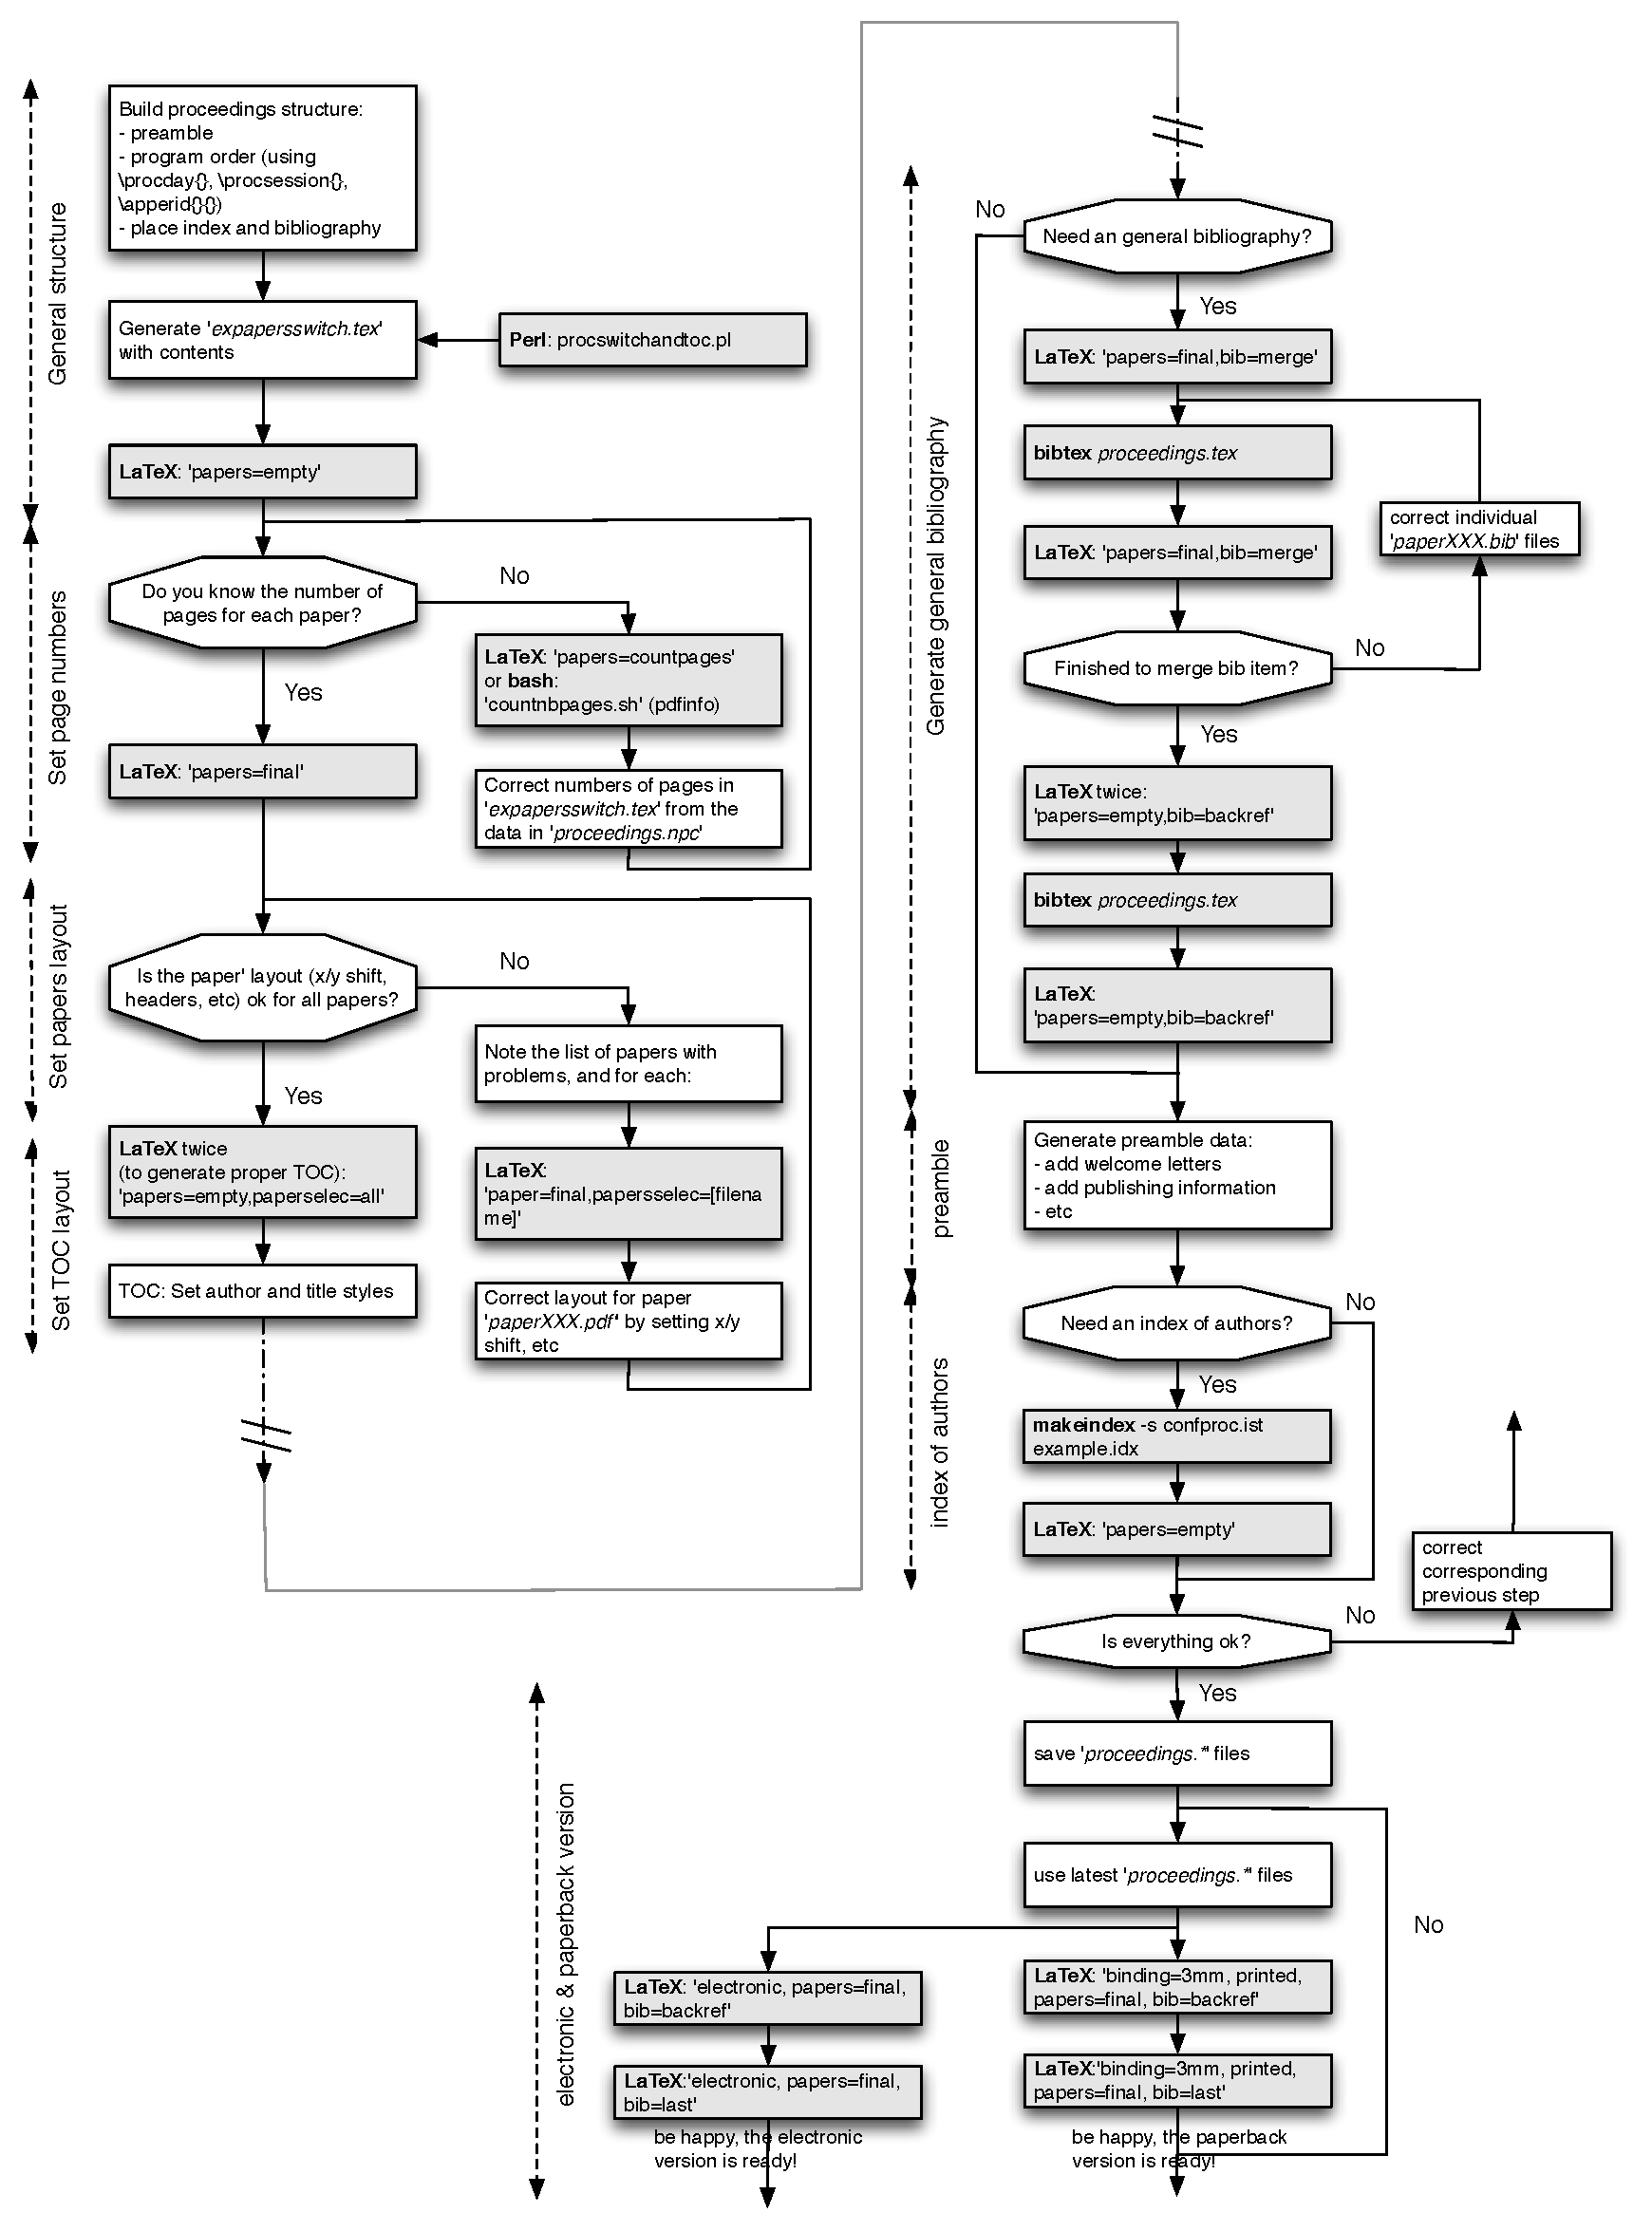
\includegraphics[width=\textwidth]{confproc_diag.pdf} 
	   \caption{Suggested stages to build proceedings}
	   \label{fig:confproc_diag}
\end{figure}


%=================================================================
\section{Compatibility with other packages}

The `confproc' package has been successfully tested with \TeX{}Live 2008, 2009 \& 2010.

%------------------------------------------------------------------------
\subsection{Essential packages required by \package{\filename}}

\begin{itemize}
  \item \LaTeXe\ ($\ge$ 1994/12/01) and pdfTeXk Version 3.1415926-1.40.9 (Web2C 7.5.7)\\
    \ctan: \href{http://www.ctan.org/tex-archive/macros/latex/base}{macros/latex/base}
  \item \package{book}
             ($\ge$ 2005/09/16 v1.4f): standard document class on which \package{\filename} is based; \\
    \ctan:  \href{http://www.ctan.org/tex-archive/macros/latex/unpacked/}{macros/latex/unpacked/}
  \item \package{kvoptions} and \package{kvoptions-patch}
             ($\ge$ 2009/04/10 v3.1): \\
    \ctan:  \href{http://www.ctan.org/tex-archive/macros/latex/contrib/oberdiek/kvoptions.dtx}{macros/latex/contrib/oberdiek/kvoptions.dtx}
  \item \package{xifthen}
             ($\ge$ 2009/04/17 v1.3): 
    \ctan:  \href{http://www.ctan.org/tex-archive/macros/latex/contrib/xifthen/}{macros/latex/contrib/xifthen/}
  \item \package{pdfpages}
             ($\ge$ 2009/02/07 v0.4g): 
    \ctan:  \href{http://www.ctan.org/tex-archive/macros/latex/contrib/pdfpages/pdfpages.dtx}{macros/latex/contrib/pdfpages/pdfpages.dtx}
  \item \package{hyperref} 
             ($\ge$ 2009/05/01 v6.78r):
    \ctan:  \href{http://www.ctan.org/tex-archive/macros/latex/contrib/hyperref/hyperref.dtx}{macros/latex/contrib/hyperref/hyperref.dtx}
   \item \package{geometry}
             ($\ge$ 2008/12/21 v4.2): 
 	           \ctan:  \href{http://www.ctan.org/tex-archive/macros/latex/contrib/geometry/geometry.dtx}{macros/latex/contrib/geometry/geometry.dtx}
  \item \package{color}
             ($\ge$ 2005/11/14 v1.0j): 
    \ctan:  \href{http://www.ctan.org/tex-archive/macros/latex/required/graphics/color.dtx}{macros/latex/required/graphics/color.dtx}
  \item \package{fancyhdr}
             ($\ge$ 2005/03/22 v3.2): 
    \ctan:  \href{http://www.ctan.org/tex-archive/macros/latex/contrib/fancyhdr/fancyhdr.sty}{macros/latex/contrib/fancyhdr/fancyhdr.sty}
  \item \package{index}
             ($\ge$ 2004/01/20 v4.2beta): 
    \ctan:  \href{http://www.ctan.org/tex-archive/macros/latex/contrib/index/index.dtx}{macros/latex/contrib/index/index.dtx}
  \item \package{tocbibind}
             ($\ge$ 2003/03/13 v1.5g): 
    \ctan:  \href{http://www.ctan.org/tex-archive/macros/latex/contrib/tocbibind/tocbibind.dtx}{macros/latex/contrib/tocbibind/tocbibind.dtx}
  \item \package{titletoc}
             ($\ge$ 2007/08/12 v1.6): 
    \ctan:  \href{http://www.ctan.org/tex-archive/macros/latex/contrib/titlesec/titletoc.sty}{macros/latex/contrib/titlesec/titletoc.sty}
  \item \package{multitoc}
             ($\ge$ 1999/06/08 v2.01): 
    \ctan:  \href{http://www.ctan.org/tex-archive/macros/latex/contrib/ms/multitoc.dtx}{macros/latex/contrib/ms/multitoc.dtx}
  \item \package{multicol}
             ($\ge$ 2006/05/18 v1.6g): 
    \ctan:  \href{http://www.ctan.org/tex-archive/macros/latex/required/tools/multicol.dtx}{macros/latex/required/tools/multicol.dtx}
  \item \package{sectsty}
             ($\ge$ 2002/02/25 v2.0.2): 
    \ctan:  \href{http://www.ctan.org/tex-archive/macros/latex/contrib/sectsty/sectsty.dtx}{macros/latex/contrib/sectsty/sectsty.dtx}
\end{itemize}

%------------------------------------------------------------------------
\subsection{Other packages used with \package{\filename} in the examples}

\begin{itemize}
  \item \package{hypcap}
             ($\ge$ 2006/02/20 v1.5):
    \ctan:  \href{http://www.ctan.org/tex-archive/macros/latex/contrib/oberdiek/hypcap.dtx}{macros/latex/contrib/oberdiek/hypcap.dtx}
	         \item \package{graphicx}
             ($\ge$ 1996/08/05 v1.0a):
    \ctan: \href{http://www.ctan.org/tex-archive/macros/latex/required/graphics/graphicx.dtx}{macros/latex/required/graphics/graphicx.dtx}
  \item \package{newapa}
             ($\ge$ 1991/06/13 v2.0):
    \ctan:  \href{http://www.ctan.org/tex-archive/biblio/bibtex/contrib/newapa/}{biblio/bibtex/contrib/newapa/}\
  \item \package{newapave}
             ($\ge$ 2006/07/31 v2.1),   
    \ctan:  \href{http://www.ctan.org/tex-archive/macros/latex/contrib/conferences/confproc/}{macros/latex/contrib/conferences/confproc/}
   \item \package{setspace}
             ($\ge$ 2000/12/01 v6.7):
    \ctan:  \href{http://www.ctan.org/tex-archive/macros/latex/contrib/setspace/setspace.sty}{macros/latex/contrib/setspace/setspace.sty}
   \item \package{inputenc}
             ($\ge$ 2006/05/05 v1.1b):
 	        \ctan:  \href{http://www.ctan.org/tex-archive/macros/latex/base/inputenc.dtx}{macros/latex/base/inputenc.dtx}
   \item \package{fontenc}
             ($\ge$ 2005/09/27 v1.99g): 
 	        \ctan:  \href{http://www.ctan.org/tex-archive/macros/latex/unpacked/fontenc.sty}{macros/latex/unpacked/fontenc.sty}
		  \item \package{mathptmx} 
             ($\ge$ 2005/04/12 PSNFSS-v9.2a):
     \ctan:  \href{http://www.ctan.org/tex-archive/macros/latex/required/psnfss/}{macros/latex/required/psnfss/}
   		  \item \package{nth} 
             ($\ge$ 2002/02/27):
     \ctan:  \href{http://www.ctan.org/tex-archive/macros/generic/misc/nth.sty}{macros/generic/misc/nth.sty}
   \item \package{layout}
             ($\ge$ 2000/09/25 v1.2c):
     \ctan:  \href{http://www.ctan.org/tex-archive/macros/latex/required/tools/layout.dtx}{macros/latex/required/tools/layout.dtx}
   \item \package{layouts}
             ($\ge$ 2004/10/25 v2.6c):
 	           \ctan:  \href{http://www.ctan.org/tex-archive/macros/latex/contrib/layouts/layouts.dtx}{macros/latex/contrib/layouts/layouts.dtx}
\end{itemize}


\end{document}
